\subsubsection{Toric code}
Similarly, a hypergraph product code of two ring codes can be 
generated. 

Unlike in Figure \ref{fig: surface_code}, it is also possible to draw topological
ECC graphs without colored plaquettes, by drawing it such that the data qubits are on 
edges of the graph and the ancilla qubits for Z-checks are on faces
while the ancilla qubits for X-checks lie on nodes.
This representation is called a Tanner graph \cite{tillichzemor}
and is used in Figure \ref{fig: toric_graph}.

Since the resulting Tanner graph forms a torus,
we call this code the "Toric code".

The logical operators on the toric code are loops, so a circle of 
'errors' on nodes is a logical X operator, and a circle of 'errors'
on faces is a logical Z operator.

\begin{figure}[htbp]
    \centering
    \begin{minipage}[t]{0.48\textwidth}
      \centering
      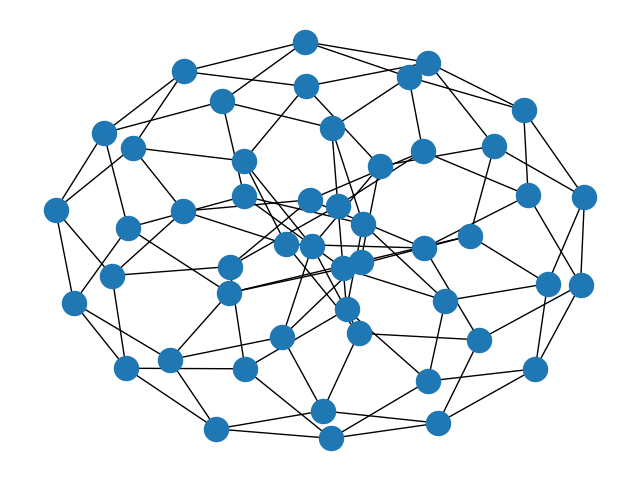
\includegraphics[width=\linewidth]{./img/figures/toric_5_graph.png}
      \caption{Tanner graph for [[49,1,7]] toric code.}
      \label{fig: toric_graph}
    \end{minipage}
    \hfill
    \begin{minipage}[t]{0.48\textwidth}
      \centering
      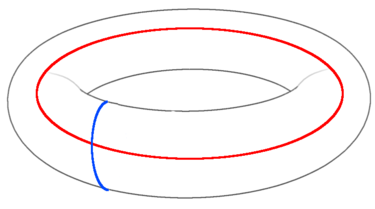
\includegraphics[width=\linewidth]{./img/figures/toriclogicals.png}
      \caption{Logical $\overline{X}$ and $\overline{Z}$ operators on toric code 
      Tanner graph. Image courtesy of James Wooton's contribution to Wikipedia.}
      \label{fig: toric logicals}
    \end{minipage}
  \end{figure}

\newpage